%%%%%%%%%%%%%
% 
% Alexander Powell
% Finite Automata
% Homework Assignment #6
% 10.22.2015
% 
%%%%%%%%%%%%%

\documentclass[11pt]{article}

\usepackage{times,mathptm}
\usepackage{pifont}
\usepackage{exscale}
\usepackage{latexsym}
\usepackage{amsmath}
\usepackage{amssymb}
\usepackage{amsthm}
\usepackage{epsfig}
\usepackage{tikz}


\textwidth 6.5in
\textheight 9in
\oddsidemargin -0.0in
\topmargin -0.0in

\parindent 0pt     % How much the first word of a paragraph is indented. 
\parskip 0pt	   % How much extra space to leave between paragraphs.

\begin{document}

\begin{center}             % If you're only centering 1 line use \centerline{}
\begin{LARGE}
{\bf Finite Automata Homework 6}
\end{LARGE}
\vskip 0.25cm      % vertical skip (0.25 cm)

Due: Thursday, Oct 22\\  % force new line
Alexander Powell
\end{center}

\begin{enumerate}

\item
Give a description and the state diagram of the PDA for the language
$$ A = \{ a^ib^jc^k | i=j \text{ or } j=k \text{ where } i,j,k \geq 0 \} $$

\textbf{Solution: }

We can describe the language $A$ as the language containing all strings of an equal number of $a's$ and $b's$ followed by some number of $c's$ and all strings containing some number of $a's$ followed by $b's$ and then $c's$, where the number of $b's$ is equal to the number of $c's$ (where any of these numbers can be $0$).  

We can write $A$ as the union of the two languages:
$$ \{ a^ib^ic^k | i,k \geq 0 \} \cup \{ a^ib^kc^k | i,k \geq 0 \} $$
The PDA for the first language can be displayed as:
\begin{center}
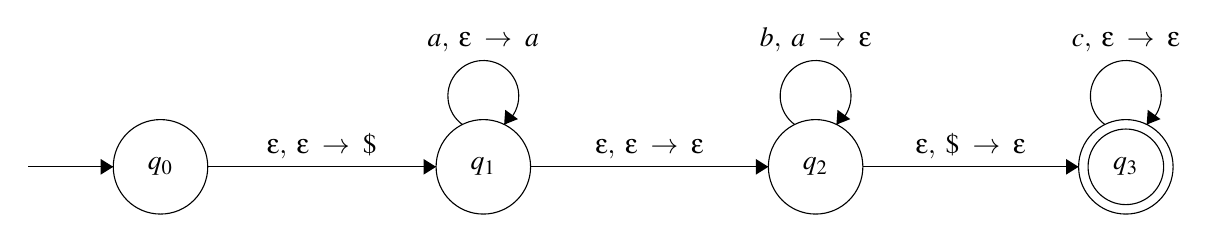
\begin{tikzpicture}[scale=0.2]
\tikzstyle{every node}+=[inner sep=0pt]
\draw [black] (9.7,-23.3) circle (3);
\draw (9.7,-23.3) node {$q_0$};
\draw [black] (30.2,-23.3) circle (3);
\draw (30.2,-23.3) node {$q_1$};
\draw [black] (51.3,-23.3) circle (3);
\draw (51.3,-23.3) node {$q_2$};
\draw [black] (71,-23.3) circle (3);
\draw (71,-23.3) node {$q_3$};
\draw [black] (71,-23.3) circle (2.4);
\draw [black] (1.3,-23.3) -- (6.7,-23.3);
\fill [black] (6.7,-23.3) -- (5.9,-22.8) -- (5.9,-23.8);
\draw [black] (12.7,-23.3) -- (27.2,-23.3);
\fill [black] (27.2,-23.3) -- (26.4,-22.8) -- (26.4,-23.8);
\draw (19.95,-22.8) node [above] {$\epsilon,\mbox{ }\epsilon\mbox{ }\rightarrow\mbox{ }\$$};
\draw [black] (33.2,-23.3) -- (48.3,-23.3);
\fill [black] (48.3,-23.3) -- (47.5,-22.8) -- (47.5,-23.8);
\draw (40.75,-22.8) node [above] {$\epsilon,\mbox{ }\epsilon\mbox{ }\rightarrow\mbox{ }\epsilon$};
\draw [black] (54.3,-23.3) -- (68,-23.3);
\fill [black] (68,-23.3) -- (67.2,-22.8) -- (67.2,-23.8);
\draw (61.15,-22.8) node [above] {$\epsilon,\mbox{ }\$\mbox{ }\rightarrow\mbox{ }\epsilon$};
\draw [black] (28.877,-20.62) arc (234:-54:2.25);
\draw (30.2,-16.05) node [above] {$a,\mbox{ }\epsilon\mbox{ }\rightarrow\mbox{ }a$};
\fill [black] (31.52,-20.62) -- (32.4,-20.27) -- (31.59,-19.68);
\draw [black] (49.977,-20.62) arc (234:-54:2.25);
\draw (51.3,-16.05) node [above] {$b,\mbox{ }a\mbox{ }\rightarrow\mbox{ }\epsilon$};
\fill [black] (52.62,-20.62) -- (53.5,-20.27) -- (52.69,-19.68);
\draw [black] (69.677,-20.62) arc (234:-54:2.25);
\draw (71,-16.05) node [above] {$c,\mbox{ }\epsilon\mbox{ }\rightarrow\mbox{ }\epsilon$};
\fill [black] (72.32,-20.62) -- (73.2,-20.27) -- (72.39,-19.68);
\end{tikzpicture}
\end{center}
The PDA for the second language can be displayed as:
\begin{center}
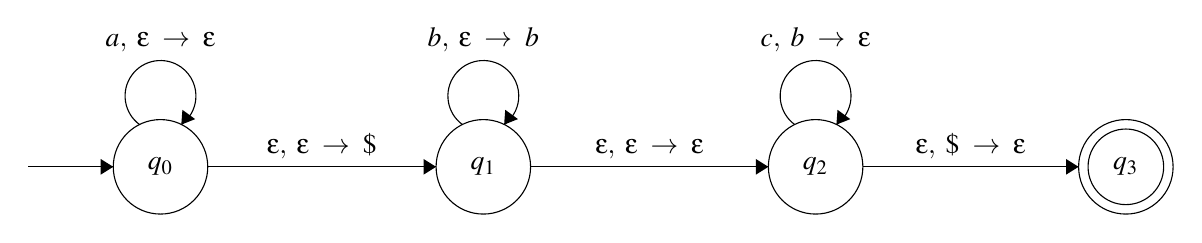
\begin{tikzpicture}[scale=0.2]
\tikzstyle{every node}+=[inner sep=0pt]
\draw [black] (9.7,-23.3) circle (3);
\draw (9.7,-23.3) node {$q_0$};
\draw [black] (30.2,-23.3) circle (3);
\draw (30.2,-23.3) node {$q_1$};
\draw [black] (51.3,-23.3) circle (3);
\draw (51.3,-23.3) node {$q_2$};
\draw [black] (71,-23.3) circle (3);
\draw (71,-23.3) node {$q_3$};
\draw [black] (71,-23.3) circle (2.4);
\draw [black] (1.3,-23.3) -- (6.7,-23.3);
\fill [black] (6.7,-23.3) -- (5.9,-22.8) -- (5.9,-23.8);
\draw [black] (12.7,-23.3) -- (27.2,-23.3);
\fill [black] (27.2,-23.3) -- (26.4,-22.8) -- (26.4,-23.8);
\draw (19.95,-22.8) node [above] {$\epsilon,\mbox{ }\epsilon\mbox{ }\rightarrow\mbox{ }\$$};
\draw [black] (33.2,-23.3) -- (48.3,-23.3);
\fill [black] (48.3,-23.3) -- (47.5,-22.8) -- (47.5,-23.8);
\draw (40.75,-22.8) node [above] {$\epsilon,\mbox{ }\epsilon\mbox{ }\rightarrow\mbox{ }\epsilon$};
\draw [black] (54.3,-23.3) -- (68,-23.3);
\fill [black] (68,-23.3) -- (67.2,-22.8) -- (67.2,-23.8);
\draw (61.15,-22.8) node [above] {$\epsilon,\mbox{ }\$\mbox{ }\rightarrow\mbox{ }\epsilon$};
\draw [black] (28.877,-20.62) arc (234:-54:2.25);
\draw (30.2,-16.05) node [above] {$b,\mbox{ }\epsilon\mbox{ }\rightarrow\mbox{ }b$};
\fill [black] (31.52,-20.62) -- (32.4,-20.27) -- (31.59,-19.68);
\draw [black] (49.977,-20.62) arc (234:-54:2.25);
\draw (51.3,-16.05) node [above] {$c,\mbox{ }b\mbox{ }\rightarrow\mbox{ }\epsilon$};
\fill [black] (52.62,-20.62) -- (53.5,-20.27) -- (52.69,-19.68);
\draw [black] (8.377,-20.62) arc (234:-54:2.25);
\draw (9.7,-16.05) node [above] {$a,\mbox{ }\epsilon\mbox{ }\rightarrow\mbox{ }\epsilon$};
\fill [black] (11.02,-20.62) -- (11.9,-20.27) -- (11.09,-19.68);
\end{tikzpicture}
\end{center}

Therefore, by putting the two state diagrams together, we get the state diagram for the PDA as a whole, shown below.  
\begin{center}
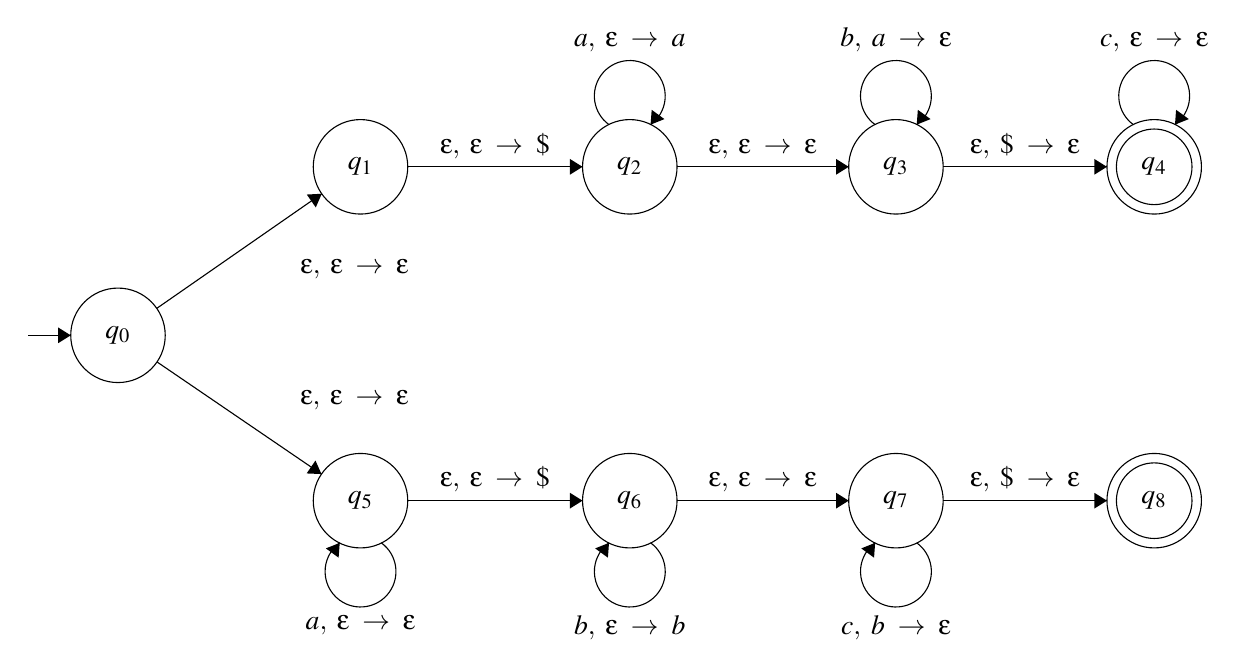
\begin{tikzpicture}[scale=0.2]
\tikzstyle{every node}+=[inner sep=0pt]
\draw [black] (21.5,-36.2) circle (3);
\draw (21.5,-36.2) node {$q_5$};
\draw [black] (38.6,-36.2) circle (3);
\draw (38.6,-36.2) node {$q_6$};
\draw [black] (55.5,-36.2) circle (3);
\draw (55.5,-36.2) node {$q_7$};
\draw [black] (71.9,-36.2) circle (3);
\draw (71.9,-36.2) node {$q_8$};
\draw [black] (71.9,-36.2) circle (2.4);
\draw [black] (6.1,-25.7) circle (3);
\draw (6.1,-25.7) node {$q_0$};
\draw [black] (21.5,-15) circle (3);
\draw (21.5,-15) node {$q_1$};
\draw [black] (38.6,-15) circle (3);
\draw (38.6,-15) node {$q_2$};
\draw [black] (55.5,-15) circle (3);
\draw (55.5,-15) node {$q_3$};
\draw [black] (71.9,-15) circle (3);
\draw (71.9,-15) node {$q_4$};
\draw [black] (71.9,-15) circle (2.4);
\draw [black] (24.5,-36.2) -- (35.6,-36.2);
\fill [black] (35.6,-36.2) -- (34.8,-35.7) -- (34.8,-36.7);
\draw (30.05,-35.7) node [above] {$\epsilon,\mbox{ }\epsilon\mbox{ }\rightarrow\mbox{ }\$$};
\draw [black] (41.6,-36.2) -- (52.5,-36.2);
\fill [black] (52.5,-36.2) -- (51.7,-35.7) -- (51.7,-36.7);
\draw (47.05,-35.7) node [above] {$\epsilon,\mbox{ }\epsilon\mbox{ }\rightarrow\mbox{ }\epsilon$};
\draw [black] (58.5,-36.2) -- (68.9,-36.2);
\fill [black] (68.9,-36.2) -- (68.1,-35.7) -- (68.1,-36.7);
\draw (63.7,-35.7) node [above] {$\epsilon,\mbox{ }\$\mbox{ }\rightarrow\mbox{ }\epsilon$};
\draw [black] (39.923,-38.88) arc (54:-234:2.25);
\draw (38.6,-43.45) node [below] {$b,\mbox{ }\epsilon\mbox{ }\rightarrow\mbox{ }b$};
\fill [black] (37.28,-38.88) -- (36.4,-39.23) -- (37.21,-39.82);
\draw [black] (56.823,-38.88) arc (54:-234:2.25);
\draw (55.5,-43.45) node [below] {$c,\mbox{ }b\mbox{ }\rightarrow\mbox{ }\epsilon$};
\fill [black] (54.18,-38.88) -- (53.3,-39.23) -- (54.11,-39.82);
\draw [black] (22.823,-38.88) arc (54:-234:2.25);
\draw (21.5,-43.45) node [below] {$a,\mbox{ }\epsilon\mbox{ }\rightarrow\mbox{ }\epsilon$};
\fill [black] (20.18,-38.88) -- (19.3,-39.23) -- (20.11,-39.82);
\draw [black] (0.4,-25.7) -- (3.1,-25.7);
\fill [black] (3.1,-25.7) -- (2.3,-25.2) -- (2.3,-26.2);
\draw [black] (8.56,-23.99) -- (19.04,-16.71);
\fill [black] (19.04,-16.71) -- (18.09,-16.76) -- (18.66,-17.58);
\draw (21.13,-20.85) node [below] {$\epsilon,\mbox{ }\epsilon\mbox{ }\rightarrow\mbox{ }\epsilon$};
\draw [black] (8.58,-27.39) -- (19.02,-34.51);
\fill [black] (19.02,-34.51) -- (18.64,-33.65) -- (18.08,-34.47);
\draw (21.12,-30.45) node [above] {$\epsilon,\mbox{ }\epsilon\mbox{ }\rightarrow\mbox{ }\epsilon$};
\draw [black] (24.5,-15) -- (35.6,-15);
\fill [black] (35.6,-15) -- (34.8,-14.5) -- (34.8,-15.5);
\draw (30.05,-14.5) node [above] {$\epsilon,\mbox{ }\epsilon\mbox{ }\rightarrow\mbox{ }\$$};
\draw [black] (41.6,-15) -- (52.5,-15);
\fill [black] (52.5,-15) -- (51.7,-14.5) -- (51.7,-15.5);
\draw (47.05,-14.5) node [above] {$\epsilon,\mbox{ }\epsilon\mbox{ }\rightarrow\mbox{ }\epsilon$};
\draw [black] (58.5,-15) -- (68.9,-15);
\fill [black] (68.9,-15) -- (68.1,-14.5) -- (68.1,-15.5);
\draw (63.7,-14.5) node [above] {$\epsilon,\mbox{ }\$\mbox{ }\rightarrow\mbox{ }\epsilon$};
\draw [black] (37.277,-12.32) arc (234:-54:2.25);
\draw (38.6,-7.75) node [above] {$a,\mbox{ }\epsilon\mbox{ }\rightarrow\mbox{ }a$};
\fill [black] (39.92,-12.32) -- (40.8,-11.97) -- (39.99,-11.38);
\draw [black] (54.177,-12.32) arc (234:-54:2.25);
\draw (55.5,-7.75) node [above] {$b,\mbox{ }a\mbox{ }\rightarrow\mbox{ }\epsilon$};
\fill [black] (56.82,-12.32) -- (57.7,-11.97) -- (56.89,-11.38);
\draw [black] (70.577,-12.32) arc (234:-54:2.25);
\draw (71.9,-7.75) node [above] {$c,\mbox{ }\epsilon\mbox{ }\rightarrow\mbox{ }\epsilon$};
\fill [black] (73.22,-12.32) -- (74.1,-11.97) -- (73.29,-11.38);
\end{tikzpicture}
\end{center}

\item
Convert $G_4$ to equivalent PDA using the procedure in theorem $2.20$.  $G_4$ is given below:
$$ E \rightarrow E + T | T $$
$$ T \rightarrow T \times F | F $$
$$ F \rightarrow (E) | a $$

\textbf{Solution: }

\begin{center}
\begin{tikzpicture}[scale=0.2]
\tikzstyle{every node}+=[inner sep=0pt]
\draw [black] (10.8,-12.8) circle (3);
\draw (10.8,-12.8) node {$q_0$};
\draw [black] (30.6,-12.8) circle (3);
\draw (30.6,-12.8) node {$q_1$};
\draw [black] (49.4,-12.8) circle (3);
\draw (49.4,-12.8) node {$q_2$};
\draw [black] (68.2,-12.8) circle (3);
\draw (68.2,-12.8) node {$q_3$};
\draw [black] (68.2,-12.8) circle (2.4);
\draw [black] (3.8,-12.8) -- (7.8,-12.8);
\fill [black] (7.8,-12.8) -- (7,-12.3) -- (7,-13.3);
\draw [black] (13.8,-12.8) -- (27.6,-12.8);
\fill [black] (27.6,-12.8) -- (26.8,-12.3) -- (26.8,-13.3);
\draw (20.7,-13.3) node [below] {$\epsilon,\mbox{ }\epsilon\mbox{ }\rightarrow\mbox{ }\$$};
\draw [black] (33.6,-12.8) -- (46.4,-12.8);
\fill [black] (46.4,-12.8) -- (45.6,-12.3) -- (45.6,-13.3);
\draw (40,-13.3) node [below] {$\epsilon,\mbox{ }\epsilon\mbox{ }\rightarrow\mbox{ }E$};
\draw [black] (52.4,-12.8) -- (65.2,-12.8);
\fill [black] (65.2,-12.8) -- (64.4,-12.3) -- (64.4,-13.3);
\draw (58.8,-13.3) node [below] {$\epsilon,\mbox{ }\$\mbox{ }\rightarrow\mbox{ }\epsilon$};
\draw [black] (50.723,-15.48) arc (54:-234:2.25);
\draw (49.4,-20.05) node [below] {\begin{tabular}{l} $\epsilon,\mbox{ }E\mbox{ }\rightarrow\mbox{ }E\mbox{ }+\mbox{ }T$ \\ $\epsilon,\mbox{ }E\mbox{ }\rightarrow\mbox{ }T$ \\ $\epsilon,\mbox{ }T\mbox{ }\rightarrow\mbox{ }T\mbox{ }\times\mbox{ }F$ \\ $\epsilon,\mbox{ }T\mbox{ }\rightarrow\mbox{ }F$ \\ $\epsilon,\mbox{ }F\mbox{ }\rightarrow\mbox{ }(E)$ \\ $\epsilon,\mbox{ }F\mbox{ }\rightarrow\mbox{ }a$ \\ $+,\mbox{ }+\mbox{ }\rightarrow\mbox{ }\epsilon$ \\ $\times,\mbox{ }\times\mbox{ }\rightarrow\mbox{ }\epsilon$ \\ $(,\mbox{ }(\mbox{ }\rightarrow\mbox{ }\epsilon$ \\ $),\mbox{ })\mbox{ }\rightarrow\mbox{ }\epsilon$ \\ $a,\mbox{ }a\mbox{ }\rightarrow\mbox{ }\epsilon$ \end{tabular}};
\fill [black] (48.08,-15.48) -- (47.2,-15.83) -- (48.01,-16.42);
\end{tikzpicture}
\end{center}

\newpage
\item
Let CFG $G$ be the grammar below:
$$ S \rightarrow aSb | bY | Ya $$
$$ Y \rightarrow bY | aY | \epsilon $$
Give a simple description of the grammar and give CFG for the complement, $\overline{L(G)}$.  

\textbf{Solution: }

$L(G)$ generates all strings over $\{ a,b \}$ such that each string begins with $n$ $a's$ and ends with $n$ $b's$ (and $n$ can be $0$).  Also, each word has either a $b$ followed by any combination of $a's$ and $b's$ or has any combination of $a's$ and $b's$ followed by an $a$ on the inside of the string.  Therefore, the grammar for the complement of the language can be written as 
$$ S \rightarrow aSb | bSa | aSa | bSb | ba $$

\item
Let $\Sigma = \{ a,b \}$.  Give the CFG generating the language of strings with twice as many $a's$ as $b's$.  

\textbf{Solution: }

To create a grammar for this language, we simply need to make sure everytime a $b$ is added to the string, two $a's$ are added along with it.  The context free grammar can be written as:
$$ S \rightarrow SS | aSaSb | aSbSa | bSaSa | \epsilon $$
%$$ S \rightarrow SS | aaSb | abSa | baSa | \epsilon $$

\item
Let $E = \{ a^ib^j | i \neq j \text{ and } 2i \neq j \}$.  Show that $E$ is a context free language.  

\textbf{Solution: }

We can rewrite the language as the union of three languages.  These are written as:
$$ \{ a^ib^j | i > j \} \cup \{ a^ib^j | i < j \text{ and } 2i > j \} \cup \{ a^ib^j | 2i < j \} $$
The first of these languages can be generated with the context free grammar below:
$$ S_1 \rightarrow aA_1B_1 $$
$$ A_1 \rightarrow aA_1 | \epsilon $$
$$ B_1 \rightarrow aB_1b | \epsilon $$
The third language can be represented with the grammar below:
$$ S_3 \rightarrow A_3B_3b $$
$$ A_3 \rightarrow aA_3bb | \epsilon $$
$$ B_3 \rightarrow B_3b | \epsilon$$
Finally, we can represent the middle grammar with the following production rules.  
$$ S_2 \rightarrow aA_2b $$
$$ A_2 \rightarrow aA_2b | aA_2bb | abb $$

\newpage
So, by putting these three grammars together to generate the union of all three languages, we get the following context free grammar.  
$$ S \rightarrow S_1 | S_2 | S_3 $$
$$ S_1 \rightarrow aA_1B_1 $$
$$ A_1 \rightarrow aA_1 | \epsilon $$
$$ B_1 \rightarrow aB_1b | \epsilon $$
$$ S_2 \rightarrow aA_2b $$
$$ A_2 \rightarrow aA_2b | aA_2bb | abb $$
$$ S_3 \rightarrow A_3B_3b $$
$$ A_3 \rightarrow aA_3bb | \epsilon $$
$$ B_3 \rightarrow B_3b | \epsilon$$

\end{enumerate}
\end{document}














